%%%%%%%%%%%%%%%%%%%%%%%%%%%%%%%%%%%%%%
% START ADDING TEXT HERE 
%
% Feel free to use \include commands to structure text in smaller
% pieces 
% 
%%%%%%%%%%%%%%%%%%%%%%%%%%%%%%%%%%%%%%


% Abstract gives a brief summary of the main points of a paper:
\begin{abstract}
  This paper gives a brief overview of the use of pigeon as a physical
  layer underlying  the IP protocol. 
\end{abstract}

% the actual content, usually separated over a number of sections
% each section is assigned a label, in order to be able to put a
% crossreference to it

\section{Introduction}
\label{sec:introduction}

The introduction describes the problem, why it is important, the main
ideas of the following paper, what are the main contributions of the
paper, etc. 

% Note: for a SEMINAR, Related Work usually is a BAD idea and makes no
% sense! 
\section{Some section}
\label{sec:relwork}

Use section labels for references, e.g., to

Section~\ref{sec:introduction}, that offer competing solutions, etc.

All sources must be properly referenced, ideally by using the
BiBTeX/Biber system. References can then be very conveniently made
with the \texttt{\\cite} command. For example, reference
\cite{leuwen00:_handb_schol} discusses some of the elementary rules on
writing scientific papers, amongst others how to correctly cite other
documents.  Lot's of other sources exist to help with writing
\cite{williams16:_style} or research in general
\cite{booth16:_craft_resear}.

Reference~\cite{Taylor:SIGuide:95}, e.g., describes how to
correctly use the SI system of units and their correct typographical
representation.


\section{Some other section}
\label{sec:model}


Such a section could, among other things, include a figure. Note that
a figure is a so-called floating object: it is moved around the actual
text in order to best fit on a page. This is in stark contrast to some
GUI-based word processing tools, where the placement of figures is
usually more associated with luck than principle.

As figures float around, expressions like ``the following figure''
must never be used. Instead, figures need a caption, a label, and must
be properly referenced in the main text. An example for this concept
is shown in Figure~\ref{fig:example}. 

\begin{figure}[htbp]
  \begin{center}
    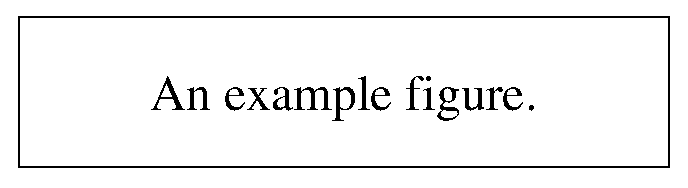
\includegraphics[width=\columnwidth]{example}
    \caption{An example figure with a caption.}
    \label{fig:example}
  \end{center}
\end{figure}

In general, only vector graphics in PDF or (possibly) encapsulated
postscript (eps) format should be included in any kind of text, as
this allows arbirary scaling, rotation etc.\ without any loss of
quality. Bitmap formats (PNG, JPEG, GIF, \dots) should only be used if no
other alternative exists --- e.g., when including photographs. 

\section{Word processing \& \LaTeX}
\label{sec:latex} 

This document has already introduced the most important constructs of
\LaTeX. What is necessary to produce documents with \LaTeX is simple
any normal text editor and a \LaTeX distribution. This is commonly
installed on practically all UNIX-type systems; for Windows, an
excellent \LaTeX exists, called MikTeX, available from
\url{www.miktex.org}. Almost all distributions come with a large patch
of examples and introductory material; consult your local installation
for details. 

Lots of supplementary and background information, FAQs, etc.\ is
available from the Comprehensive TeX Archive Network (CTAN); the
German mirror of which is \url{www.dante.de}. 


\section{Just some text}
\label{sec:just-some-text}

Just some text to show pagination etc. 

Pellentesque dapibus suscipit ligula.  Donec posuere augue in quam.  Etiam vel tortor sodales tellus ultricies commodo.  Suspendisse potenti.  Aenean in sem ac leo mollis blandit.  Donec neque quam, dignissim in, mollis nec, sagittis eu, wisi.  Phasellus lacus.  Etiam laoreet quam sed arcu.  Phasellus at dui in ligula mollis ultricies.  Integer placerat tristique nisl.  Praesent augue.  Fusce commodo.  Vestibulum convallis, lorem a tempus semper, dui dui euismod elit, vitae placerat urna tortor vitae lacus.  Nullam libero mauris, consequat quis, varius et, dictum id, arcu.  Mauris mollis tincidunt felis.  Aliquam feugiat tellus ut neque.  Nulla facilisis, risus a rhoncus fermentum, tellus tellus lacinia purus, et dictum nunc justo sit amet elit.

Nullam eu ante vel est convallis dignissim.  Fusce suscipit, wisi nec facilisis facilisis, est dui fermentum leo, quis tempor ligula erat quis odio.  Nunc porta vulputate tellus.  Nunc rutrum turpis sed pede.  Sed bibendum.  Aliquam posuere.  Nunc aliquet, augue nec adipiscing interdum, lacus tellus malesuada massa, quis varius mi purus non odio.  Pellentesque condimentum, magna ut suscipit hendrerit, ipsum augue ornare nulla, non luctus diam neque sit amet urna.  Curabitur vulputate vestibulum lorem.  Fusce sagittis, libero non molestie mollis, magna orci ultrices dolor, at vulputate neque nulla lacinia eros.  Sed id ligula quis est convallis tempor.  Curabitur lacinia pulvinar nibh.  Nam a sapien.

Aliquam erat volutpat.  Nunc eleifend leo vitae magna.  In id erat non orci commodo lobortis.  Proin neque massa, cursus ut, gravida ut, lobortis eget, lacus.  Sed diam.  Praesent fermentum tempor tellus.  Nullam tempus.  Mauris ac felis vel velit tristique imperdiet.  Donec at pede.  Etiam vel neque nec dui dignissim bibendum.  Vivamus id enim.  Phasellus neque orci, porta a, aliquet quis, semper a, massa.  Phasellus purus.  Pellentesque tristique imperdiet tortor.  Nam euismod tellus id erat.

\section{Math}
\label{sec:math}

\(a+b=\sqrt{c}\ = \int \sin(x) \mathrm{d}x \) 


\section{Tables}
\label{sec:tables}

Tables  like Table~\ref{tab:example}; they float and should be typeset using the booktabs package (see
documentation there). 


\begin{table}[htbp]
  \centering
  \begin{tabular}{ll}
    \toprule 
    a & b \\
    \midrule 
    c & d \\
    e & f \\
    \bottomrule
  \end{tabular}
  \caption{Example table}
  \label{tab:example}
\end{table}


\section{ PERFORMANCE EVALUATION}
\label{sec:pet-peeves}

\begin{itemize}

\item Simulation on NSFNET and ARPANET topologies
\item Results were compared with other methods.
\item Performance DDPG and DRL-TE was evaluated for each network topologies.

\subsection{Factors for comparisons}
\label{sec:orgheadline1}
\begin{itemize}

\item End to end delay
\item End to end throughput.
\item Total Utility.

\end{itemize}

\end{itemize}

\section{Conclusion}
\label{sec:concl}

At the end, there is a final section \emph{concluding} a paper,
putting the entire work into perspective and explaining, on a larger
level, what the consequences of this work are. Also, unexpected
results can be discussed here, etc.

Putting a \emph{summary} at the end is a common, yet bad practice. Try
to avoid it; it is just boring. 

 